With the state-space model of the HDT defined, the next step is to design a control strategy that ensures the desired performance. 

\begin{figure}[t!]
    \centering
    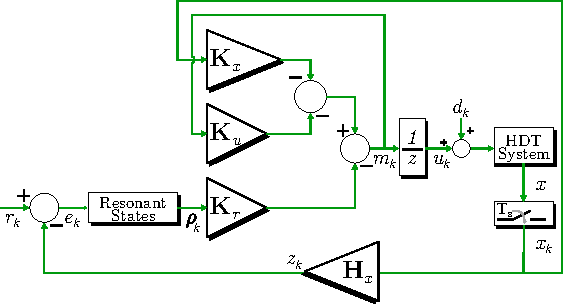
\includegraphics[width=\columnwidth]{Images/Control_Diagram.pdf} 
    \caption{Block diagram of the proposed control strategy for the HDT.}
    \label{fig:Control_Diagram}
\end{figure}

\begin{figure*}[t!]
    \centering
    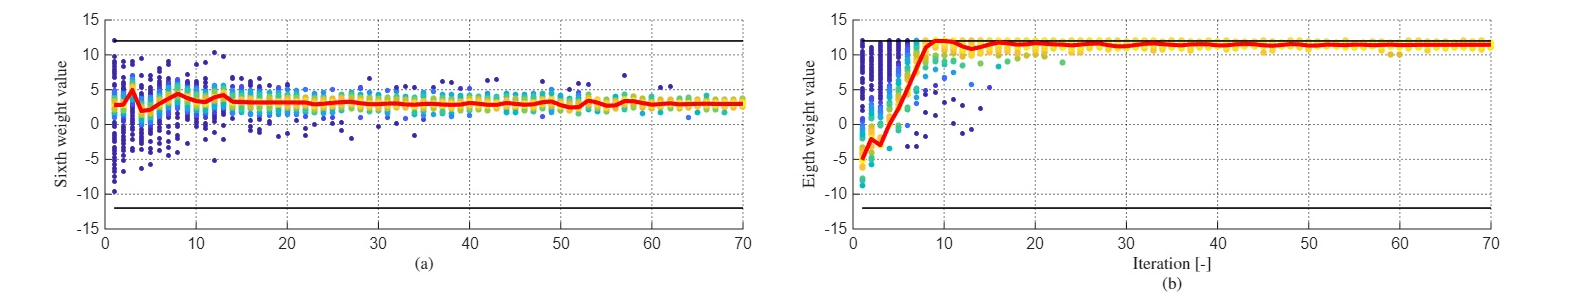
\includegraphics[width = \textwidth]{Images/w6_w8_iterations.pdf}
    \caption{Convergence of exponents over the PSO iterations. (a) Exponent $q_6$ associated with the parallel converter inductor current $v_{cp,\alpha\beta}$. (b) Exponent $q_8$ associated with the first resonant state of the error $e1v_{cs,\alpha\beta}$.}
    \label{fig:PSO_Convergence}
\end{figure*}

\subsection{Proposed Control Strategy}

The proposed control strategy is based on a state feedback controller which is designed using the augmented state-space model of the HDT, defined in \eqref{eq:AugmentedModel}. The control strategy aims to achieve zero steady-state error for sinusoidal references. For that reason, the system is expanded using the following resonant terms:
\begin{equation}
    \dot{\rho}_1 = 
    \underbrace{
    \begin{bmatrix}
        0 & \omega \\
        -\omega & 0
    \end{bmatrix}
    }_{\mathbf{A}_{r1}}
    \rho_1 + 
    \underbrace{
    \begin{bmatrix}
        1\\
        0
    \end{bmatrix}
    }_{\mathbf{B}_{r1}}
    e_1
\end{equation}
where $\omega$ is the nominal angular frequency, $\rho_1$ and $e$ are the first resonant and error components respectively. Each of the references signals has two resonant states associated with it, meaning that for the HDT control, there are eight resonant states in total (4 for the $ev_{cs,\alpha\beta}$ and 4 for the $i_{fp,\alpha\beta}$). This can be expressed as:
\begin{align}
    \begin{aligned}
        \dot{\rho} &= \underbrace{\text{diag}(\mathbf{A}_{r1}, \mathbf{A}_{r1} \mathbf{A}_{r1}, \mathbf{A}_{r1})}_{\mathbf{A}_{r}}\rho\\
        &+ \underbrace{\text{diag}(\mathbf{B}_{r1}, \mathbf{B}_{r1}, \mathbf{B}_{r1}, \mathbf{B}_{r1})}_{\mathbf{B}_{r}}e\label{eq:ResonantTerms}
    \end{aligned}
\end{align}

These resonant states are then discretized using a ZOH giving the matrices $\mathbf{A}_{rd}$ and $\mathbf{B}_{rd}$. Hence, the expanded system that includes the augmented state-space defined in \eqref{eq:AugmentedModel} and the resonant terms defined in \eqref{eq:ResonantTerms} is defined as:

\begin{align}
    \begin{aligned}
        \begin{bmatrix}
            x_{k + 1}\\
            u_{k + 1}\\
            \rho_{k + 1}
        \end{bmatrix}
        &=
        \underbrace{
        \begin{bmatrix}
            \mathbf{A}_{d,delay} & \mathbf{0} \\
            \mathbf{B}_{rd}\mathbf{H}_x & \mathbf{A}_{rd}
        \end{bmatrix}
        }_{\mathbf{A}_{d,\text{aug}}}
        \begin{bmatrix}
            x_k\\
            u_k\\
            \rho_k
        \end{bmatrix}
        +
        \underbrace{
        \begin{bmatrix}
            \mathbf{B}_{d,\text{delay}}\\
            \mathbf{0}
        \end{bmatrix}
        }_{\mathbf{B}_{d,\text{aug}}}
        \begin{bmatrix}
            m_k\\
            r_k
        \end{bmatrix}
        \\
        y_k &= 
        \begin{bmatrix}
            \mathbf{C} & \mathbf{0}
        \end{bmatrix}
        \begin{bmatrix}
            x_k\\
            u_k\\
            \rho_k
        \end{bmatrix}, \quad
        e_k = r_k - \mathbf{H}_x x_k
    \end{aligned}
\end{align}
where the matrix $\mathbf{H}_x$ selects the states with reference following and $r_k$ is the reference vector.
Then, the state feedback controller is designed using the discrete LQR approach given by:
\begin{equation}
    \mathbf{K} = \text{dlqr}(\mathbf{A}_{d,\text{aug}}, \mathbf{B}_{d,\text{aug}}, \mathbf{Q}, \mathbf{R})
\end{equation}
where $\mathbf{Q}\in\mathbb{R}^{11}$ and $\mathbf{R}\in\mathbb{R}^4 = \mathbf{I}$ are the state and input weighting matrices, respectively. The gain matrix is partitioned into three sub-matrices: $\mathbf{K}_x$, $\mathbf{K}_u$ and $\mathbf{K}_r$ for convenience. The block diagram of the proposed control strategy is shown in \Cref{fig:Control_Diagram}. With the partitioned gain matrices defined, the control input can be expressed as:
\begin{equation}
    m_k = -\mathbf{K}_x
    x_k - \mathbf{K}_u u_k - \mathbf{K}_r \rho_k
\end{equation}
where $\mathbf{K}_x$ is the state feedback gain matrix, $\mathbf{K}_u$ is the previous control input gain matrix and $\mathbf{K}_r$ is the resonant states gain matrix.

The series converter reference is calculated as the difference between the nominal value of the grid voltage and the actual value and the parallel converter reference is the sum of the DC-link control loop, which uses the instantaneous power theory~\cite{akagiControlStrategyActive1986}, and the harmonic elimination control loop. This is based in the work from Carreno et al.~\cite{carrenoStateFeedbackControlHybrid2024}.

\subsection{Particle Swarm Optimization}

To facilitate the tuning of the state feedback gain matrix $\mathbf{K}$ by adjusting $\mathbf{Q}$, the PSO algorithm is employed to optimize the weights associated with each state in the cost function. The PSO algorithm is a population-based optimization technique inspired by the social behavior of birds and fish~\cite{clercSwarmQueenDeterministic1999}. It consists of a swarm of particles, where each particle represents a potential solution to the optimization problem, in this case, the vector of powers $q_{x,j}(i)$, where $x$, $j$ and $i$ are the state, particle and iteration numbers. The particles move through the search space, updating their positions based on their own experience and the experience of their neighbors. The velocity and position of each particle are updated using the following equations:
\begin{align}
    \begin{aligned}
        v_j(i + 1) &= K_{ap}\left(v_j(i) + c_1 r_1 (pbest_j - x_j(i)) \right.\\
        & \left. + c_2 r_2 (gbest - x_j(i))\right)\\
        x_j(i + 1) &= x_j(i) + v_j(i + 1)
    \end{aligned}
\end{align}
where $v_j(i)$, $x_j(i)$, $pbest_j$ and $gbest$ are the velocity, position, the best position and global-best position of the particle $j$ at iteration $i$. $c_1$ and $c_2$ are cognitive and social acceleration coefficients, $r_1$ and $r_2$ are random numbers uniformly distributed in the range [0, 1], and $K_{ap}$ is the constriction factor given by:
\begin{equation}
    K_{ap} = \dfrac{2}{\left|2 - \phi - \sqrt{\phi^2 - 4\phi}\right|}
\end{equation}
where $\phi = c_1 + c_2 > 4$ is a constant that ensures convergence.

The PSO algorithm iteratively updates the positions and velocities of the particles until the maximum of iteration number is reached. The best position found by the swarm is considered the optimal solution to the optimization problem.

\subsection{PSO Performance Index}

The performance index used for the PSO optimization is a cost function that considers both the transient and steady-state performance of the HDT~\cite{ufnalskiParticleSwarmOptimization2015}. This index is minimized through many iterations considering the HDT system with step of sinusoidal references and without any applied disturbances. The cost function is defined as:
\begin{equation}
    J = \dfrac{1}{N} \sum_{i=1}^{N} |e_k|^2 + \beta \Delta u_k^2
\end{equation}
where $N$ is the number of samples in the simulation, $\Delta u_k$ is the change in control input at sample $k$, and $\beta$ is a weighting factor that balances the importance of the transient and steady-state performance, which is the only parameter that should be tuned according to the simulation results from the iterations process.

The assumptions that are made when running the PSO algorithm is that the penalties for the $\alpha$ and $\beta$ components are equal, including the resonant terms for each of the components. For that reason, the search of space is shrunk from the 22 states to the half. Also, to simplify the search space of the swarm, the particles are applied as powers of the state weights. This can be expressed as:
\begin{equation}
    \mathbf{Q} = \text{diag}\left\{10^{q_1}\mathbf{I}, 10^{q_2}\mathbf{I}, ..., 10^{q_{11}}\mathbf{I}\right\}
\end{equation}
The optimization variables lie within a define range including the absorbing walls boundaries~\cite{robinsonParticleSwarmOptimization2004} which allows obtaining a not-large LQR gain. The PSO parameters used for the optimization are listed in \Cref{tab:PSO_Parameters}.

\begin{table}[t!]
    \centering
    \caption{PSO parameters used for the optimization of the control gains.}
    \label{tab:PSO_Parameters}
    \begin{tabular}{|l|c|}
        \hline
        \textbf{Parameter} & \textbf{Value}\\
        \hline\hline
        Number of particles & 100\\
        Maximum number of iterations & 70\\
        Maximum weight exponent for states & $[-20, 20]$\\
        Absorbing walls boundaries & $[-12, 12]$\\
        Cognitive acceleration coefficients ($c_1$, $c_2$) & 2.05\\
        Performance index weighting factor ($\beta$) & $2\times10^{-7}$\\
        \hline
    \end{tabular}
\end{table}

\begin{table}[h!]
    \centering
    \caption{Optimized state weight exponents $q_i$ from PSO.}
    \label{tab:PSO_Weights}
    \begin{tabular}{|c|c|c|c|c|c|}
        \hline
        $q_1$ & $q_2$ & $q_3$ & $q_4$ & $q_5$ & $q_6$\\
        \hline
        $-6.186$ & $-7.810$ & $-4.406$ & $-1.642$ & $-8.674$ & $-5.315$\\
        \hline
        $q_7$ & $q_8$ & $q_9$ & $q_{10}$ & $q_{11}$ &\\
        \hline
        $-11.118$ & $11.999$ & $9.672$ & $10.516$ & $8.827$ & \\
        \hline
    \end{tabular}
\end{table}

After running the PSO algorithm, each of the optimal state weights exponents ($q_x$) that the algorithm found are given in the \Cref{tab:PSO_Weights}. As an example, the convergence of two of the exponents over the PSO iterations is shown in \Cref{fig:PSO_Convergence}, while the convergence of the fitness value over the PSO iterations is shown in \Cref{fig:PSO_Fitness}.


\begin{figure}[t!]
    \centering
    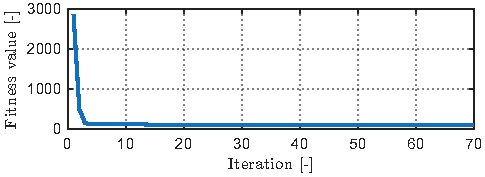
\includegraphics[]{Images/Fitness_iterations.pdf}
    \caption{Convergence of the fitness value over the PSO iterations.}
    \label{fig:PSO_Fitness}
\end{figure}

\begin{figure*}[t!]
    \centering
    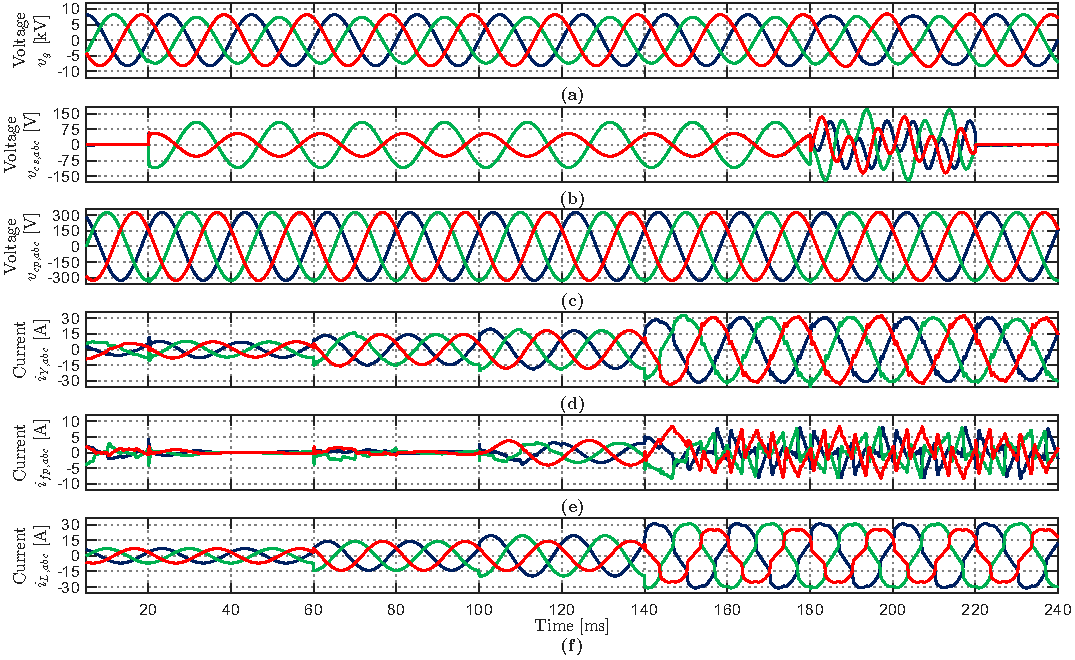
\includegraphics[width=\textwidth]{Images/Simulation_Results.pdf}
    \caption{Simulation results in $abc$ coordinates for the proposed control strategy under grid and load disturbances. (a) Grid voltage, (b) Series converter output voltage, (c) Parallel converter output voltage, (d) Secondary side transformer current, (e) Parallel converter current, (f) Load current}
    \label{fig:Sim_results}
\end{figure*}